\documentclass[hidelinks,11pt,titlepage,a4paper]{article} 
\usepackage[nottoc]{tocbibind}
\setcounter{tocdepth}{4}
\setcounter{secnumdepth}{4}
\usepackage[dvipsnames]{xcolor}
\usepackage[pdftex]{graphicx}
\usepackage{float}
\usepackage{fancyvrb}
\fvset{xleftmargin=2em}

\usepackage{pgfplots}
\pgfplotsset{width=10cm,compat=1.9}
\usepackage{tikzscale}
\usepackage{pgfplotstable}
\usepackage{booktabs}
\usepackage[font=small,labelfont=bf,tableposition=top]{caption}

\usepackage{minted}
\usemintedstyle{emacs}
\setminted{
frame=lines,
framesep=2mm,
baselinestretch=1.2,
fontsize=\footnotesize,
linenos, 
breaklines,
breakautoindent=false,
autogobble
}

\usepackage[utf8]{inputenc}
\usepackage[portuges]{babel}
% ----------------------------------------------
%Letra parecida com Arial
\usepackage{helvet}
\renewcommand{\familydefault}{\sfdefault}
\usepackage[T1]{fontenc}
% ---------------------------------------------


%\usepackage{lmodern}
\usepackage[obeyspaces,spaces]{url}
\usepackage[left=20mm,right=20mm,top=25mm,bottom=25mm]{geometry}

\usepackage{mathtools}
\usepackage{amsfonts}


\usepackage{indentfirst}
\usepackage{url}
\usepackage[]{hyperref}
\usepackage{xspace}

\hypersetup{
%pdftitle={Trabalho 1 - Gestão de Projeto},
%pdfauthor={Bruno Pereira},
%pdfsubject={Investigação Operacional},
%pdfkeywords={keyword1, keyword2}},
bookmarksnumbered=true,     
bookmarksopen=true,         
bookmarksopenlevel=1,       
colorlinks=true,            
pdfstartview=Fit,           
pdfpagemode=UseOutlines, % this is the option you were lookin for
pdfpagelayout=TwoPageRight
		}


%\usepackage{caption}
\usepackage{syntax}
\usepackage{verbatim}
\usepackage{subfig}










\newcommand{\HRule}{\rule{\linewidth}{0.5mm}}







%%%%%%%%%%%%  CABEÇALHO  %%%%%%%%%%%%%

\usepackage{fancyhdr}
\pagestyle{fancy}
\lhead{
\includegraphics[height=0.53in]{resources/template/logo-ee.png}}
\rhead{\textsl{\leftmark}}
\cfoot{\thepage}
\renewcommand{\headrulewidth}{2pt}
\renewcommand{\footrulewidth}{1pt}

%%%%%%%%%%%%%%%%%%%%%%%%%%%%%%%%%%%%%%




%Usado em conjunto com o comando \layout. Este último mostra todos os valores
%dos elementos de página.
%\usepackage{layout}

%Mostra um conjunto de quadros/frames em cada página, correspondente ao tamanho
%de cada elemento de página, como rodapé, cabeçalho, intervalos entre estes,
%margem para notas
%
%\usepackage{showframe}

%Ajusta cabeçalho para altura do logotipo
\headheight= 44pt
%Coloca margem de notas dentro da página
\marginparwidth= 40pt


%%%%%%%%%%%%%%%%%%%%%%%%%%%%%%%%%%%%%%%%%%%%%%%%%%%%%%%%%%%%%%%%%%%%%%
%%USADO EM CONJUNTO COM O PACOTE LAYOUT
%%MOSTRA ELEMENTOS DA PÁGINA, COMO CABEÇALHO, RODAPÉ, MARGEM PARA NOTAS, CORPO
%%SEPARADORES ENTRE ELEMENTOS.
%%
%%
%\begin{figure}[htbp] 
%	\begin{center} \leavevmode 
%		\layout
%		\vspace{3cm}
%		\caption{Elementos da página. Os valores mostrados são aqueles que estão
%aplicados ao presente documento, não os valores por defeito } 
%\label{fig:layout} 
%	\end{center} 
%\end{figure}
%%%%%%%%%%%%%%%%%%%%%%%%%%%%%%%%%%%%%%%%%%%%%%%%%%%%%%%%%%%%%%%%%%%%%%%%

%--- Quotes ---%
%\usepackage{epigraph}
 
%\setlength\epigraphwidth{12cm} % default 8
%\setlength\epigraphrule{0pt}

%\begin{quote}
%	
%\end{quote}
\begin{document}

%%%%%%%%%%%%%%%%%%%%%%%%%%%%%%%%%%%%%%%%%%%%

% ----------- %
\begin{titlepage}


\begin{minipage}{0.3\textwidth}
\begin{flushleft} 

\includegraphics[width=1.1\textwidth]{./resources/template/logo-ee.png}
\end{flushleft}
\end{minipage}
\hfill
\begin{minipage}{0.6\textwidth}
\begin{flushright} 

\fontfamily{pag}\selectfont{\large \textsc{Universidade do Minho}\\[0.1cm]
\large \bfseries Mestrado Integrado em Engenharia Informática \\ [0.1cm]
\large \bfseries \textit{Gestão de Redes}\\[4mm]
}
\end{flushright}
\end{minipage}\\[1cm]


\vspace{5cm}


\begin{center}



\textsc{\LARGE Trabalho Prático 3}\\[1cm]


{\Large \bfseries Implementação e desenho de servidor de números aleatórios\\[2cm]}

\vspace{1cm}
\begin{minipage}{0.7\textwidth}
\begin{center}
\minipage{0.32\textwidth}

	\begin{flushleft} 
	
\includegraphics[scale=0.3,keepaspectratio]{./resources/template/bruno.png}
	\end{flushleft}

	\begin{flushleft} 
 	\large \textbf{Bruno Pereira}\\[0.2cm]
           \texttt{a72628}
 	\end{flushleft}
\endminipage\hfill
\minipage{0.32\textwidth}
	\begin{center}
	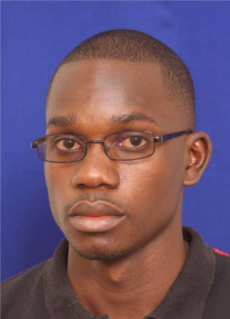
\includegraphics[scale=0.3,,keepaspectratio]{./resources/template/adriano.png}
	\end{center}

	\begin{center}
	\large \textbf{Adriano Seie}\\[0.2cm]
       	   \texttt{pg33007}
	\end{center}
 	
\endminipage\hfill
\minipage{0.32\textwidth}%
	\begin{flushright} 
	
\includegraphics[scale=0.3,,keepaspectratio]{./resources/template/marcos.png}
	\end{flushright}

	\begin{flushright} 
	\large \textbf{Marcos Andrade}\\[0.2cm]
           \texttt{a59776}
	\end{flushright}
 	
\endminipage
\end{center}
\end{minipage}





\vfill

\large Braga, {\large \today}

\end{center}
\end{titlepage}



% ----------- %
\tableofcontents
\newpage
\listoffigures
\newpage
% ----------- %


%---------------------------------------------------------------------------------------------------------------%
\section*{Introdução\markboth{\MakeUppercase{Introdução}}{}}
\addcontentsline{toc}{section}{Introdução}

\clearpage
%---------------------------------------------------------------------------------------------------------------%
\section{Fase --- A}
%---------------------------------------------------------------------------------------------------------------%

Nesta fase, requer-se que se especifique uma MIB com que implemente dois grupos:
um grupo (\texttt{unpredictableParam}) que conterá os parâmetros de
funcionamento do servidor, nomeadamente o rácio de refrescamento (\texttt{R}),
o número de entrada na tabela (\texttt{N}), o tamanho dos dígitos hexadecimais
(\texttt{D}) e, adicionalmente, um objeto escalar de cariz especial, do tipo
\emph{string} e com apenas permissões de escrita, para a operação do
\emph{reset} do agente; outro grupo (\texttt{unpredictableTable}) com a tabela
de \texttt{N} números aleatórios, onde a mesma deve incluir apenas duas colunas,
uma para o índice de entrada (chave da tabela) e outra para um número aleatório
(sequência de \texttt{D} dígitos hexadecimais).

Procedeu-se de seguida ao desenho da MIB, segundo uma árvore do OID's, onde se
decidiu que o módulo da MIB, no âmbito deste trabalho, ficasse abaixo do nodo
\emph{experimental} com o identificador 99. Adicionalmente, e para o ficheiro
ficar \emph{bem formado}, adicionou-se dois \texttt{OBJECT-GROUP} para os grupos
mencionados acima, uma vez que, cada objeto numa MIB deve ser incluído pelo
menos numa definição de grupo, seja ela, \texttt{OBJECT-GROUP} ou
\texttt{NOTIFICATION-GROUP} (RFC2580 §3.1 and §4.1). A hierarquia da árvore fica
como está na \emph{Figura~\ref{fig:fasea:arvoreoids}}. 


\begin{center}
 	
	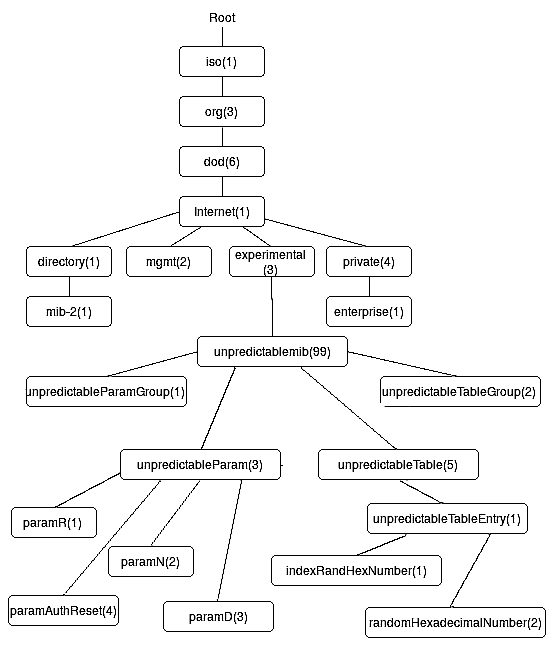
\includegraphics[scale=0.75,keepaspectratio]{resources/images/faseA/arvoreOID.png}
 	\captionsetup{type=figure, width=0.8\linewidth}
	\caption{Árvore de OIDs}
\label{fig:fasea:arvoreoids} 
\end{center}

\newpage

Em seguida procedeu-se à redação da MIB, com a consequente validação no software
\emph{MibDesigner}. Em primeiro lugar definiram as convenções textuais e tipos
de objeto a importar. Como foi anteriormente se disse, é necessário implementar
dois objetos do tipo \emph{string}: o parâmetro de autenticação para
\emph{reset} no agente e o número hexadecimal. Assim, decidiu-se importar
a convenção textual \emph{DisplayString} e o tipo \texttt{OBJECT-GROUP} (este
último justificado anteriormente). A secção de \emph{imports} pode-se ver na
figura \emph{FIgura~\ref{fig:fasea:imports}}.  

\begin{center}
 	
 	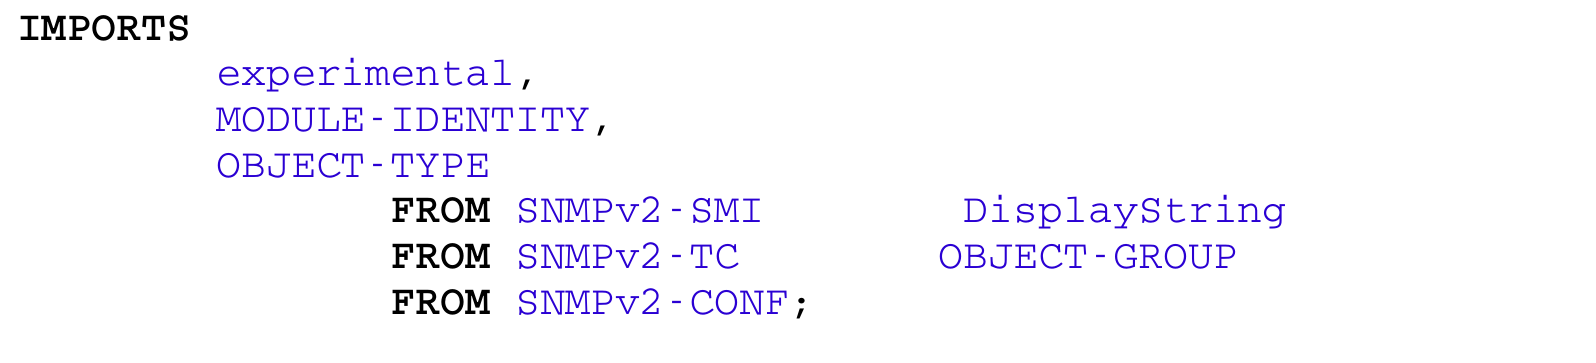
\includegraphics[width=\textwidth,height=\textheight,keepaspectratio]{resources/images/faseA/mib/imports.png}
 	\captionsetup{type=figure, width=0.8\linewidth}
	\caption{\emph{Imports} }
\label{fig:fasea:imports} 
\end{center}

\newpage

Definiu-se, também o módulo da MIB, com o nome
\texttt{unpredictableMIB}. Este tem, para além do número identificador uma série
de informações sobre quem fez o módulo, contatos, descrição e afins. A sua
definição pode ser verificada na \emph{Figura~\ref{fig:fasea:modulo}}. 

\begin{center}
 	
 	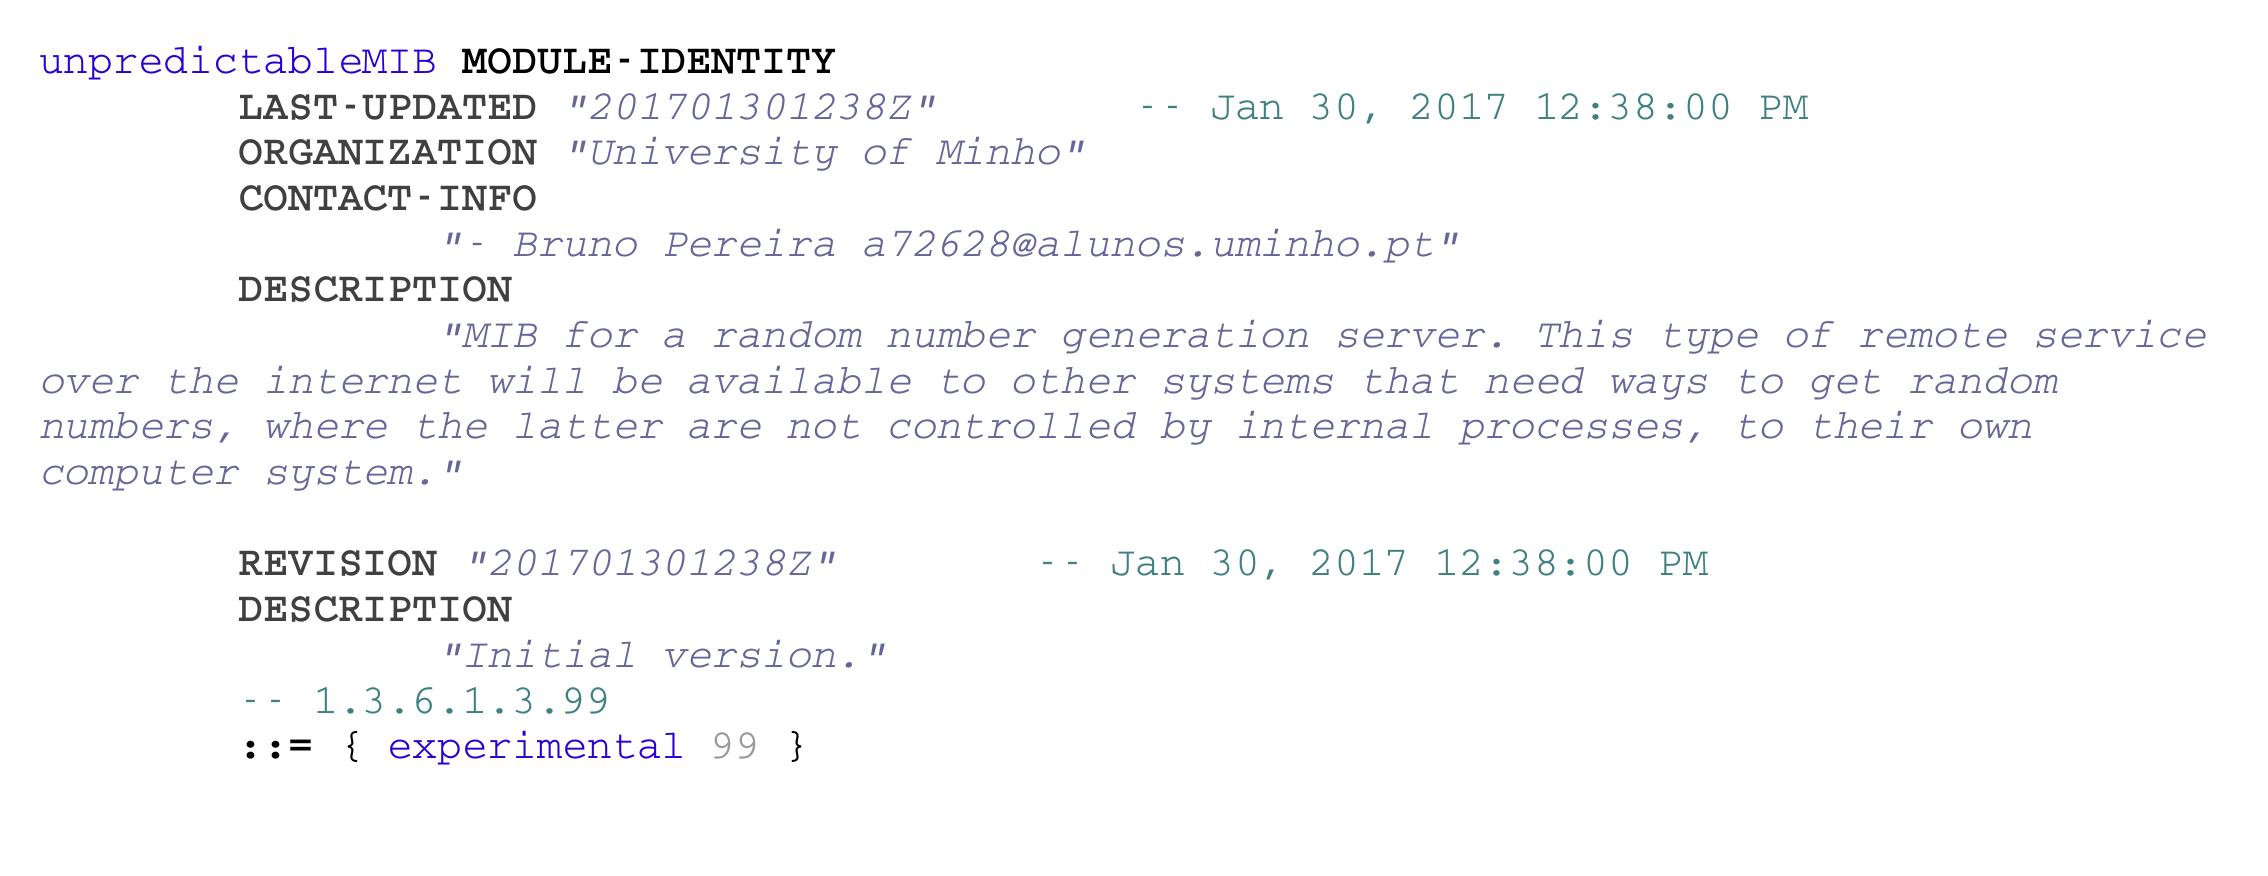
\includegraphics[width=\textwidth,height=\textheight,keepaspectratio]{resources/images/faseA/mib/modulo.png}
 	\captionsetup{type=figure, width=0.8\linewidth}
	\caption{Módulo \texttt{unpredictableMIB} }
\label{fig:fasea:modulo} 
\end{center}



Seguidamente, definiram os \texttt{OBJECT-GROUP} incluindo os objetos em cada
grupo, respetivamente. Note-se que, a ordem porque está esta declaração, tem
o intuito de declarar os grupos, como protótipos dos grupos segundo a sua
propriedade, neste caso como devem ser implementados em grupo. Adicionalmente,
criou-se um \texttt{OBJECT-IDENTIFIER} para o grupo \texttt{unpredictableParam}.
Note-se que não se fez o mesmo para o grupo \texttt{unpredictableTable} porque,
como se poderá ver em seguida, não faz sentido adicionar um nível intermédio na
árvore de OID's, uma vez que a definição do objeto tabela é um grupo.

\begin{center}
 	
 	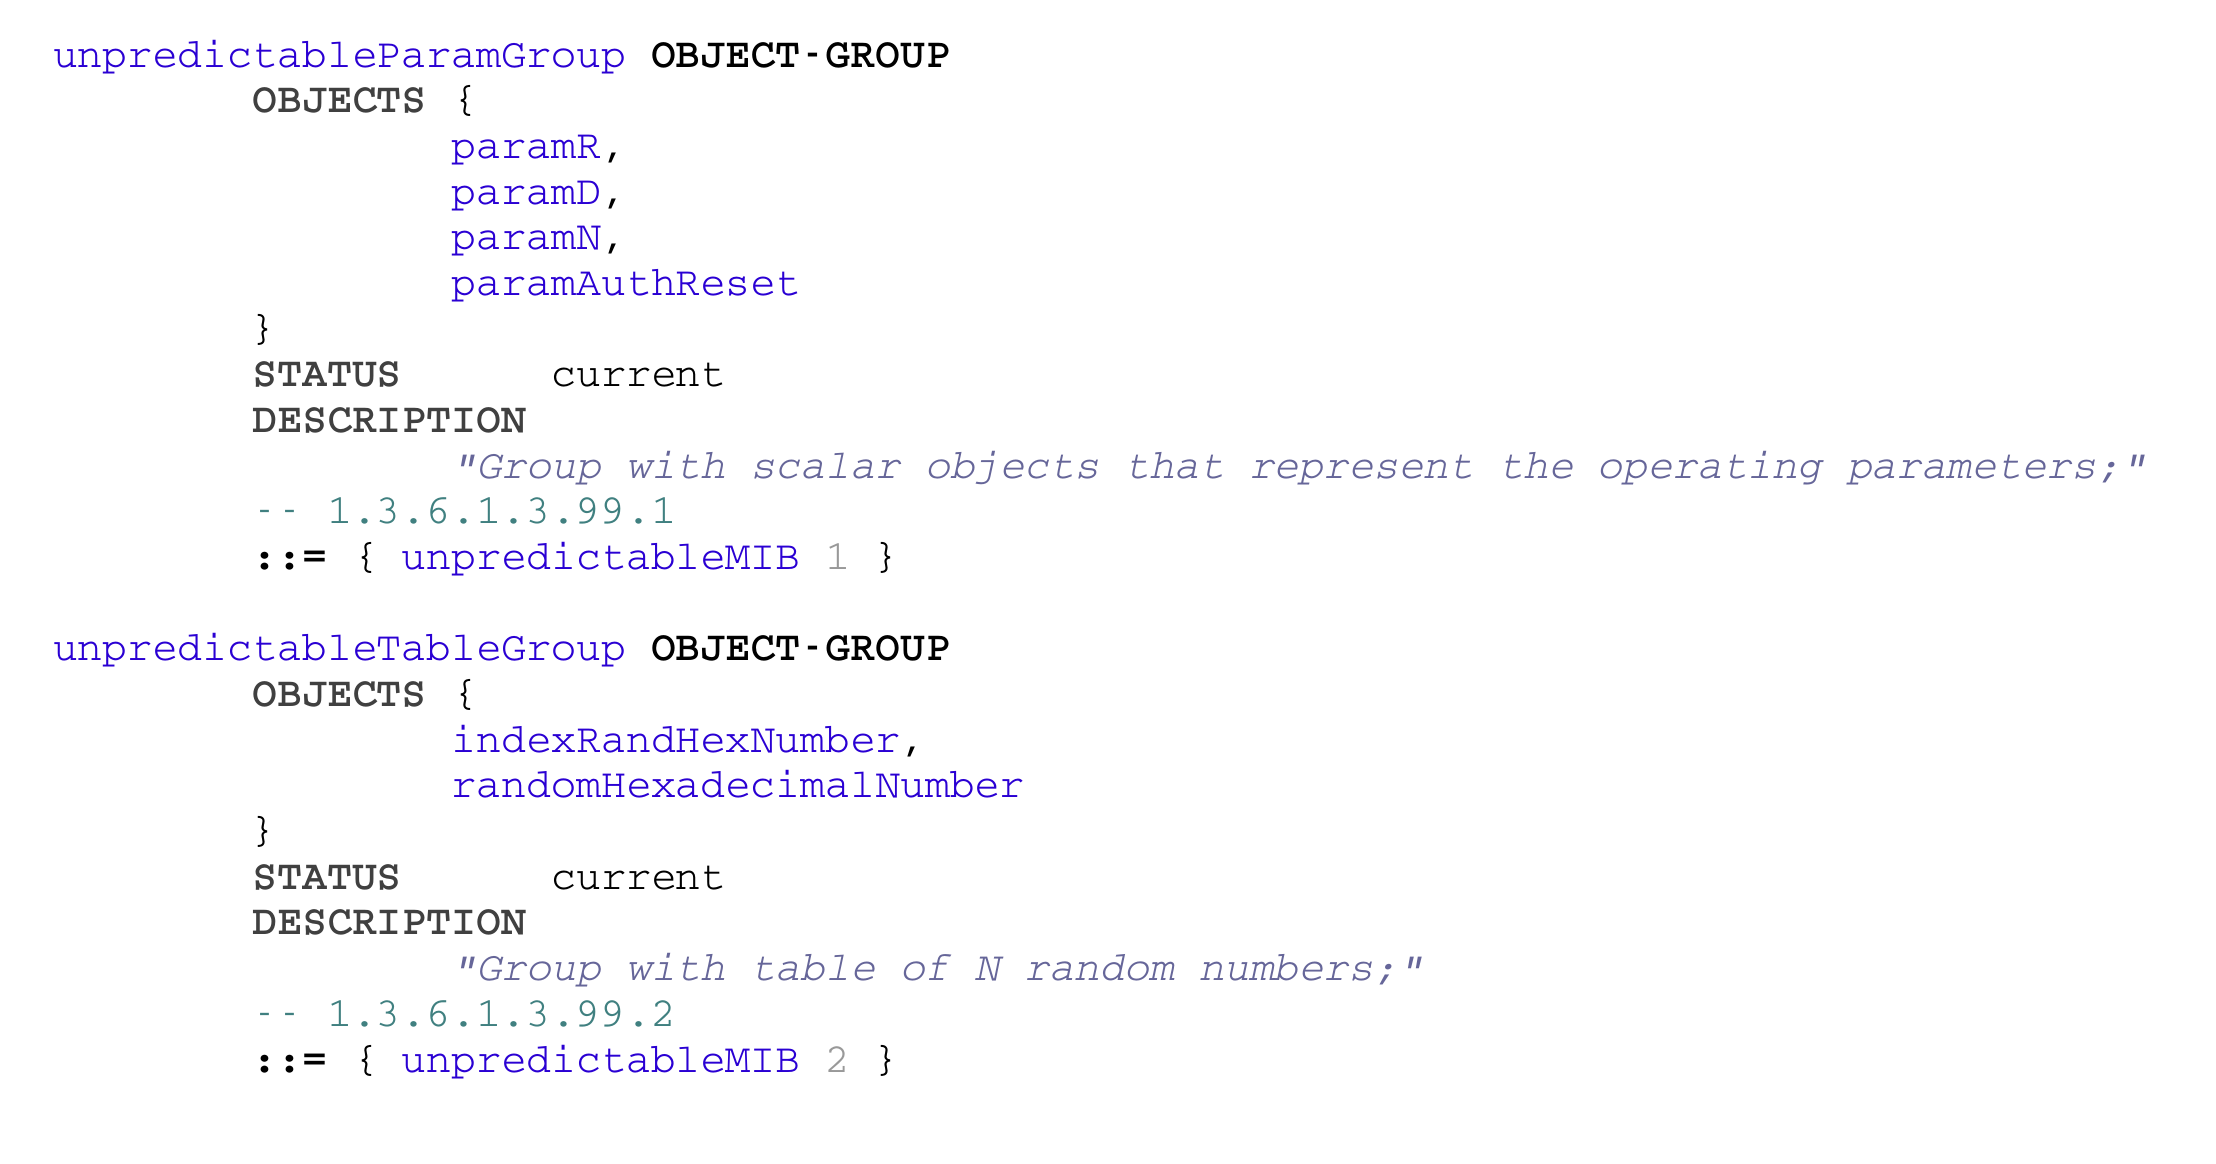
\includegraphics[width=\textwidth,height=\textheight,keepaspectratio]{resources/images/faseA/mib/groups.png}
 	\captionsetup{type=figure, width=0.8\linewidth}
	\caption{Grupos necessários}
\label{fig:fasea:groups} 
\end{center}

\newpage

\begin{center}
 	
 	
\includegraphics[width=\textwidth,height=\textheight,keepaspectratio]{resources/images/faseA/mib/scalars/groupid.png}
 	\captionsetup{type=figure, width=0.8\linewidth}
	\caption{Definição do identificador de grupo de escalares}
\label{fig:fasea:groupid} 
\end{center}

Depois adicionaram-se os escalares para os parâmetros de funcionamento do
agente. Estes objetos são todos \emph{read-only}, exceto o \emph{paramAuthReset}
que é \emph{read-write}. Note-se que o \emph{MibDesigner} não possuía a opção
\emph{write-only}, no entanto, estas definições foram depois refinadas ao nível
do código do agente, seja da definição da VACM, seja no acesso do objeto.


\begin{center}
 	
 	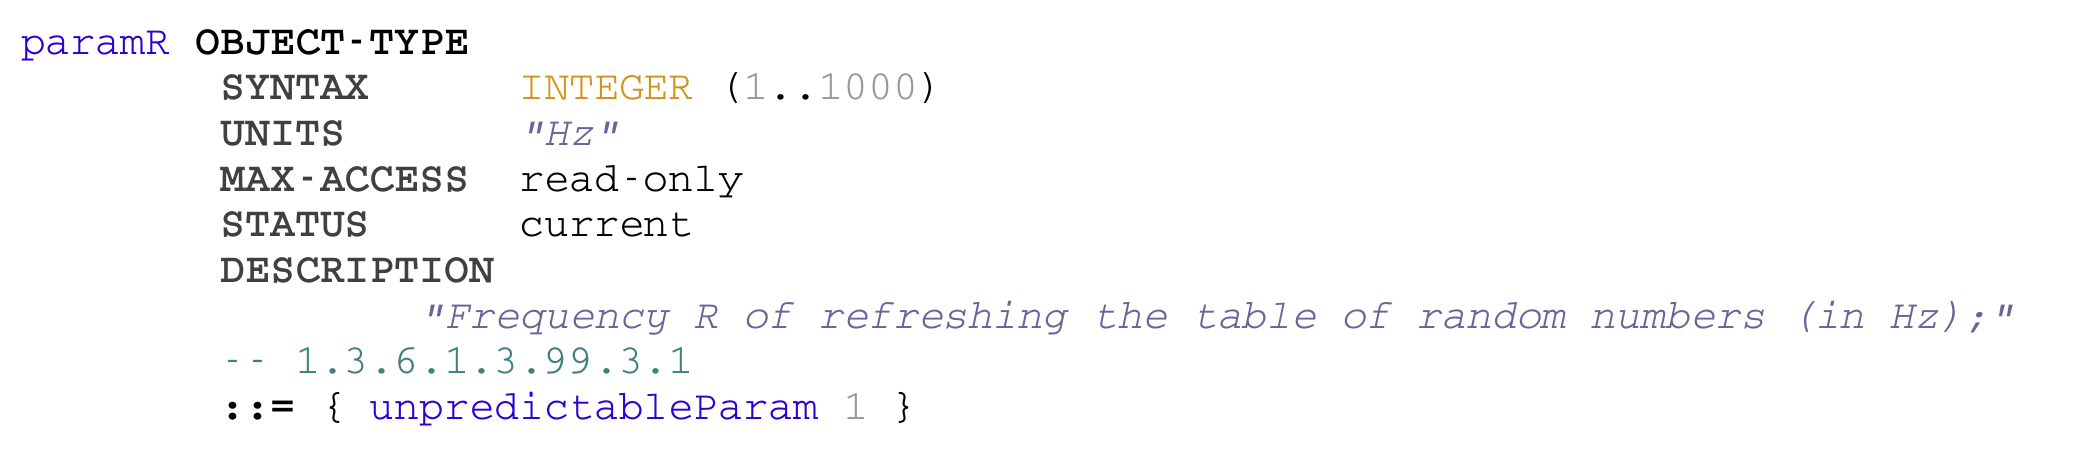
\includegraphics[width=\textwidth,height=\textheight,keepaspectratio]{resources/images/faseA/mib/scalars/paramR.png}
 	\captionsetup{type=figure, width=0.8\linewidth}
	\caption{Escalar para refrescamento (parâmetro R)}
\label{fig:fasea:} 
\end{center}

\begin{center}
 	
 	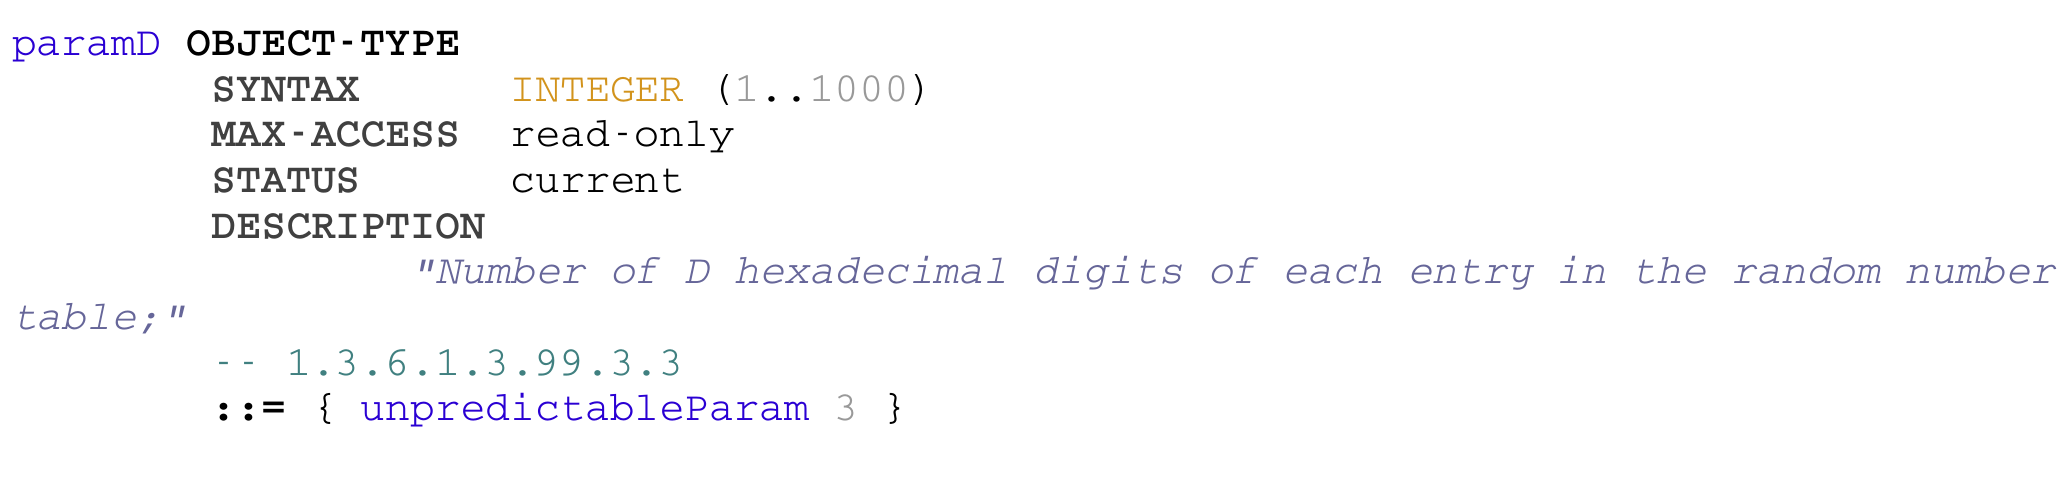
\includegraphics[width=\textwidth,height=\textheight,keepaspectratio]{resources/images/faseA/mib/scalars/paramD.png}
 	\captionsetup{type=figure, width=0.8\linewidth}
	\caption{Escalar para número de dígitos hexadecimais (parâmetro D)}
\label{fig:fasea:} 
\end{center}

\begin{center}
 	
 	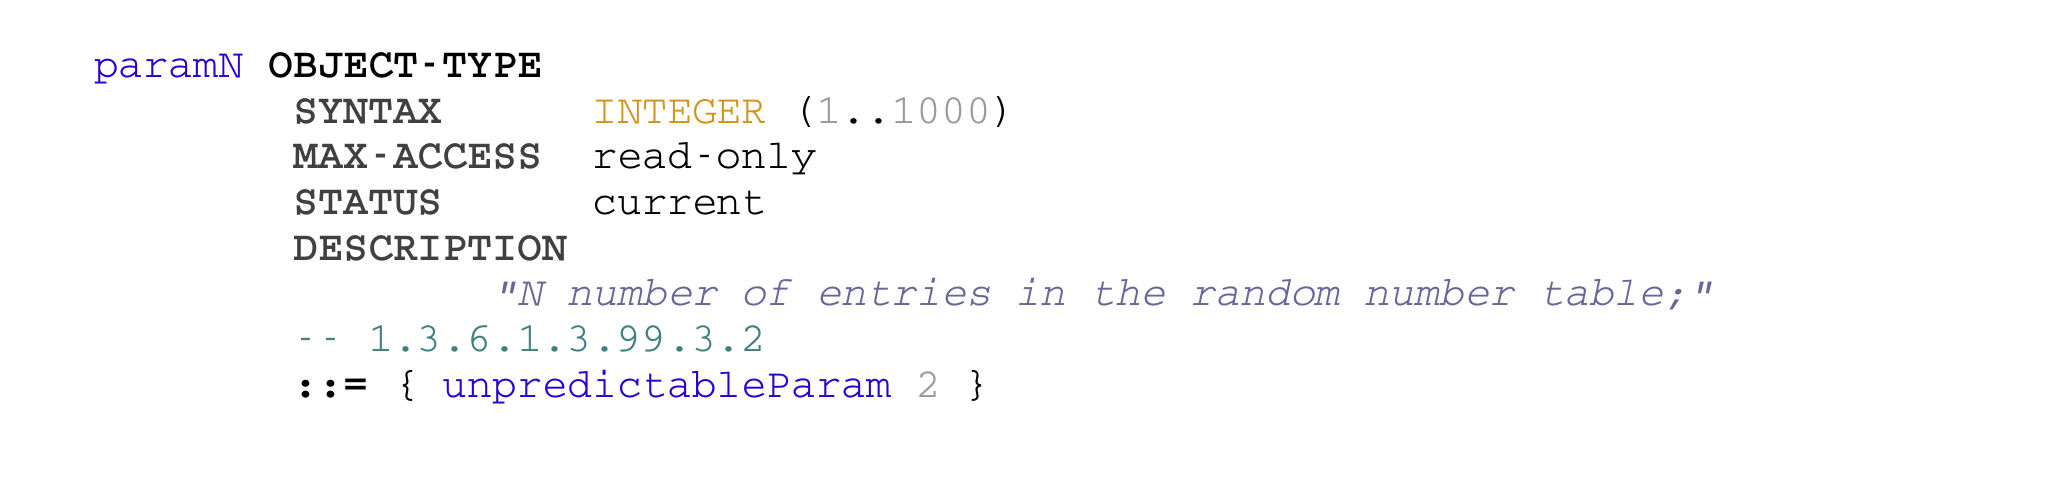
\includegraphics[width=\textwidth,height=\textheight,keepaspectratio]{resources/images/faseA/mib/scalars/paramN.png}
 	\captionsetup{type=figure, width=0.8\linewidth}
	\caption{Escalar para número de linhas da tabela (parâmetro N)}
\label{fig:fasea:} 
\end{center}

\begin{center}
 	
 	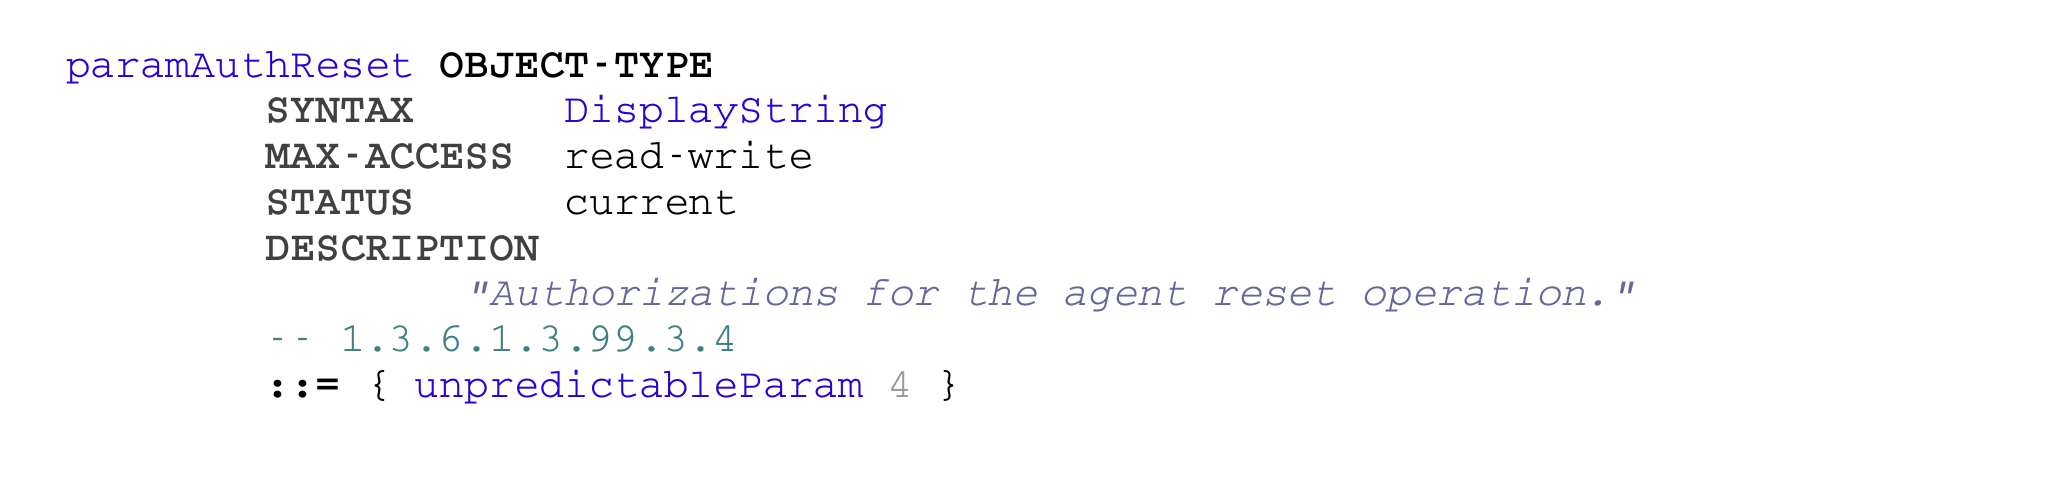
\includegraphics[width=\textwidth,height=\textheight,keepaspectratio]{resources/images/faseA/mib/scalars/paramAuthReset.png}
 	\captionsetup{type=figure, width=0.8\linewidth}
	\caption{Escalar para chave de autenticação para \emph{reset} }
\label{fig:fasea:} 
\end{center}

\newpage
A definição da tabela está na figura seguinte, e ficou definida como um
sequência de \emph{UnpredictableTableEntry}, que por sua vez é uma sequência
com o índice da tabela e o número hexadecimal associado. 

\begin{center}
 	
 	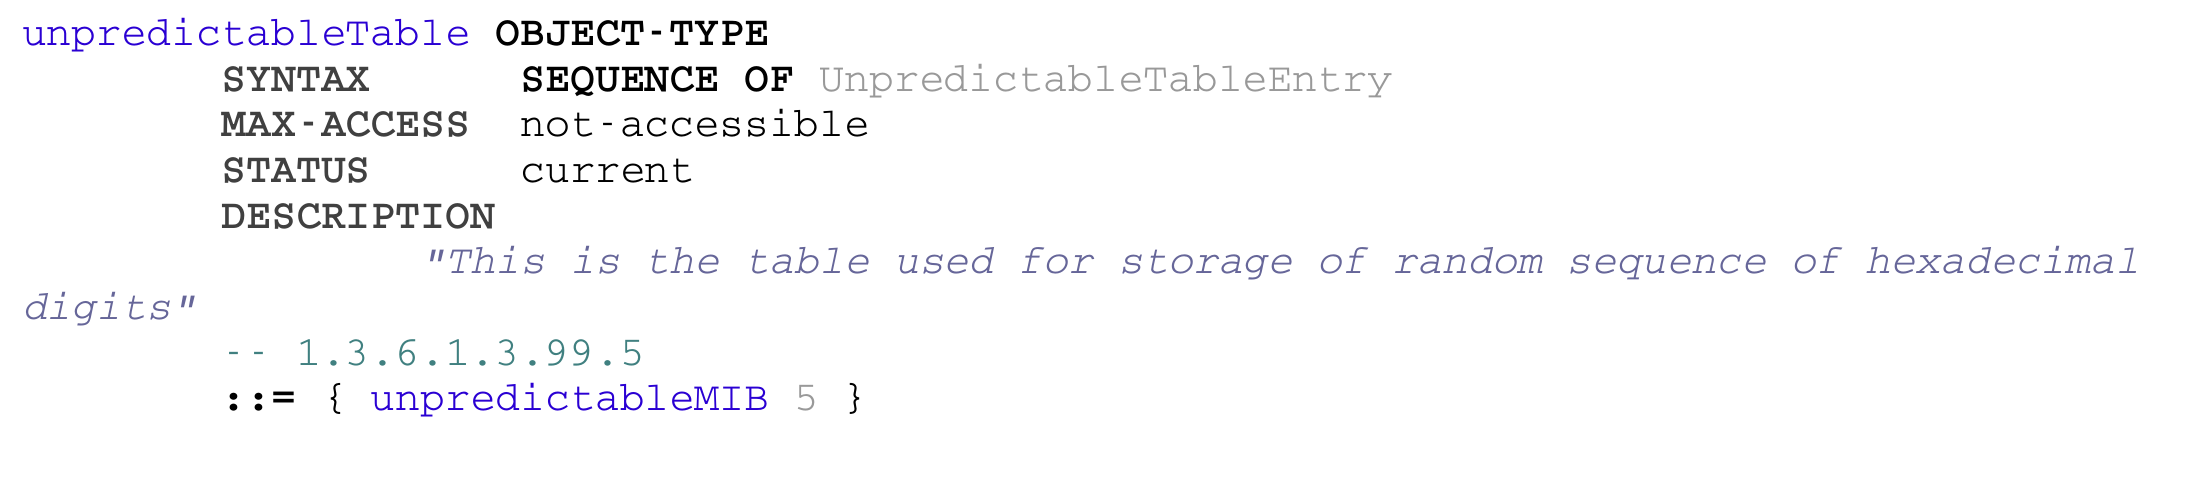
\includegraphics[width=\textwidth,height=\textheight,keepaspectratio]{resources/images/faseA/mib/tables/table.png}
 	\captionsetup{type=figure, width=0.8\linewidth}
	\caption{Identificador de grupo e da tabela}
\label{fig:fasea:} 
\end{center}

\begin{center}
 	
 	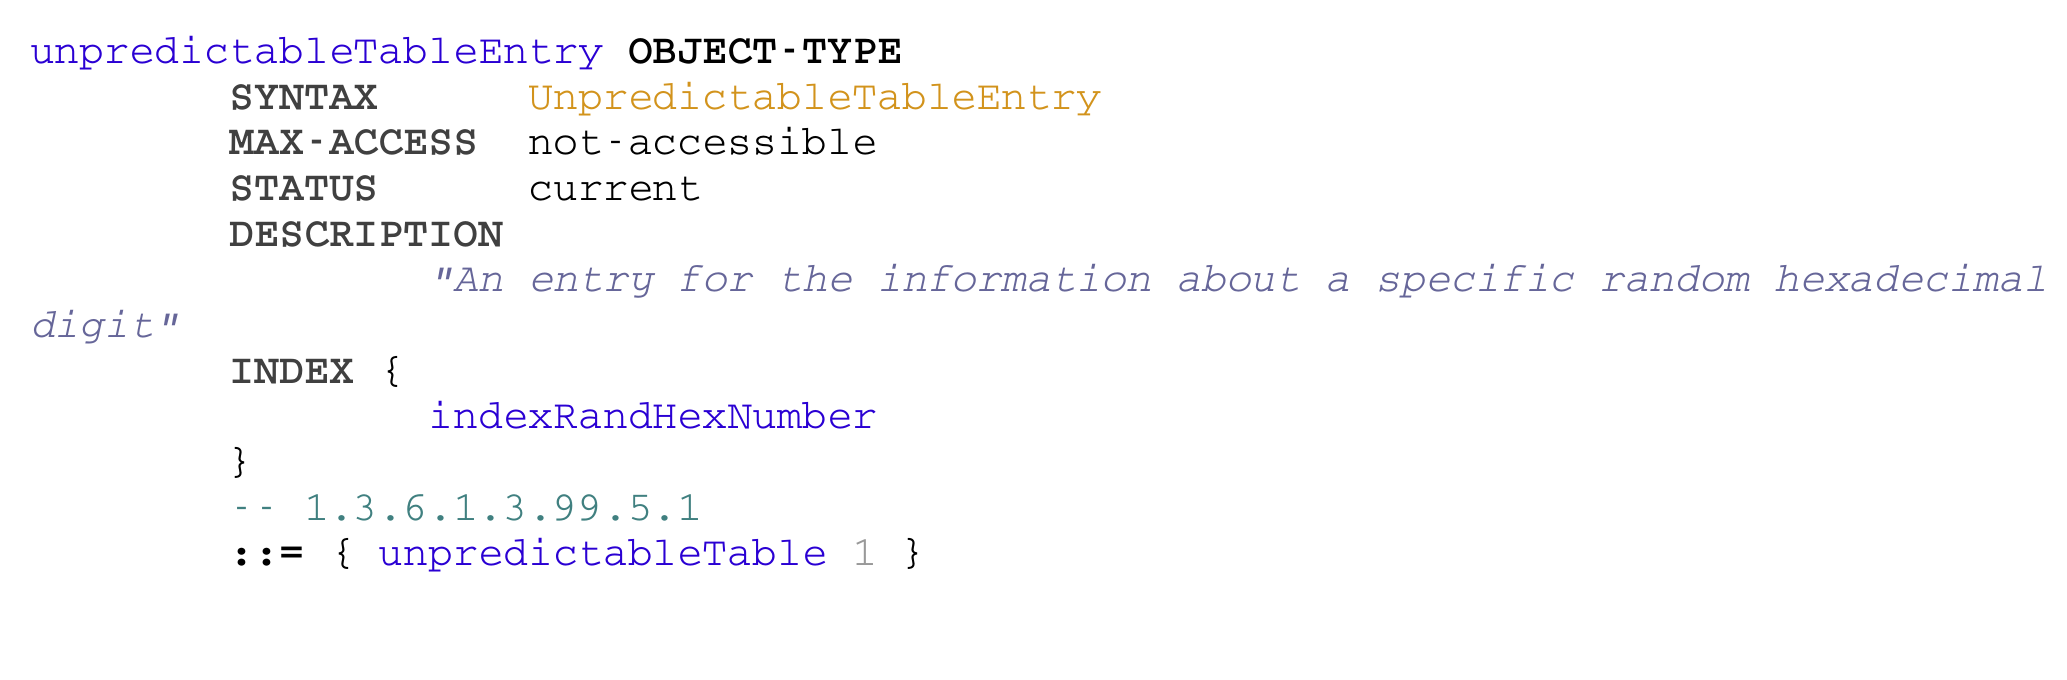
\includegraphics[width=\textwidth,height=\textheight,keepaspectratio]{resources/images/faseA/mib/tables/tableentry.png}
 	\captionsetup{type=figure, width=0.8\linewidth}
	\caption{Definição do tipo da entrada de tabela}
\label{fig:fasea:} 
\end{center}

\newpage
O objeto representativo do índice da tabela, foi definido como \emph{read-only}
e um inteiro entre 1 e 1000. Por sua vez, o objeto representativo do número
hexadecimal foi definido como \emph{read-write}, por motivos aqui já mencionados
e o seu tipo como um \emph{DisplayString}. 

\begin{center}
 	
 	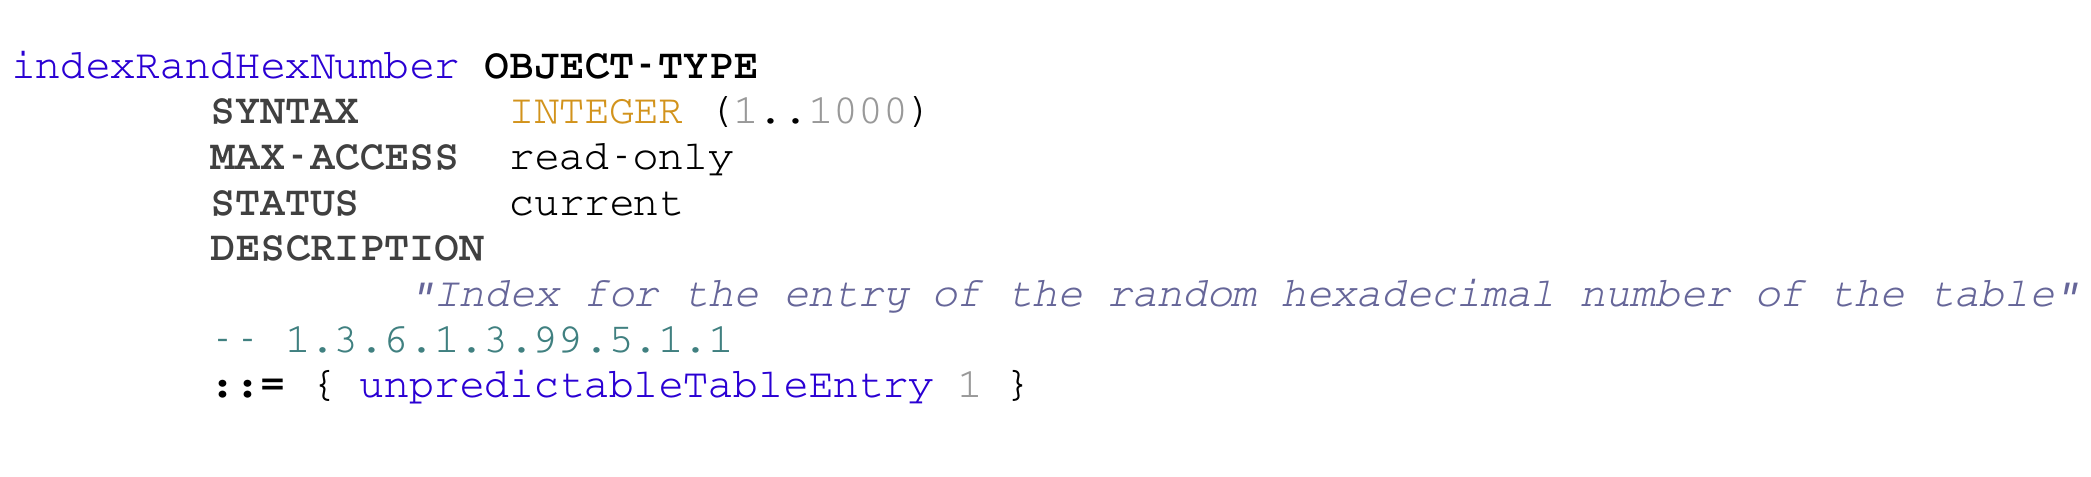
\includegraphics[width=\textwidth,height=\textheight,keepaspectratio]{resources/images/faseA/mib/tables/indextable.png}
 	\captionsetup{type=figure, width=0.8\linewidth}
	\caption{Escalar para indexação da tabela}
\label{fig:fasea:} 
\end{center}

\begin{center}
 	
 	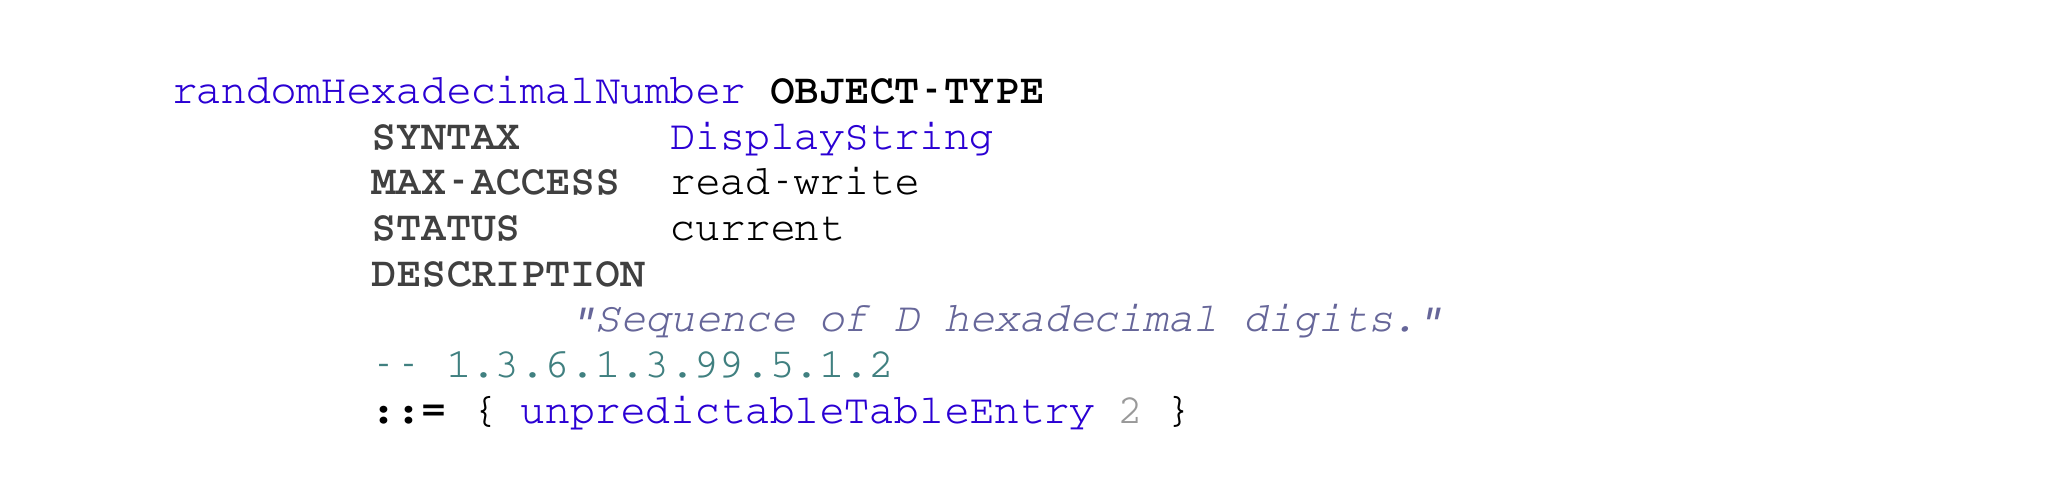
\includegraphics[width=\textwidth,height=\textheight,keepaspectratio]{resources/images/faseA/mib/tables/hexadecimalnumber.png}
 	\captionsetup{type=figure, width=0.8\linewidth}
	\caption{Escalar para representação de um número hexadecimal}
\label{fig:fasea:} 
\end{center}

\begin{center}
 	
 	
\includegraphics[width=\textwidth,height=\textheight,keepaspectratio]{resources/images/faseA/mib/tables/tableentrydefinition.png}
 	\captionsetup{type=figure, width=0.8\linewidth}
	\caption{Declaração do tipo da entrada da tabela de números hexadecimais}
\label{fig:fasea:} 
\end{center}













\clearpage
%---------------------------------------------------------------------------------------------------------------%
\section{Fase --- B}
%---------------------------------------------------------------------------------------------------------------%








\begin{center}
 	 	\begin{minted}{java}
protected void addViews(VacmMIB vacm) {

		vacm.addGroup(
			SecurityModel.SECURITY_MODEL_SNMPv2c, //Security Model
			new OctetString("c" + this.communityString), // Security Name
			new OctetString("v1v2group"), //Group Name
			StorageType.nonVolatile); // Storage type

		vacm.addAccess(
			new OctetString("v1v2group"), //Group Name
			new OctetString(this.communityString),// Context Prefix
			SecurityModel.SECURITY_MODEL_ANY, // Security Model
			SecurityLevel.NOAUTH_NOPRIV, Security Level
			MutableVACM.VACM_MATCH_EXACT, // Match
				new OctetString("fullReadView"),  // Read View
			new OctetString("fullWriteView"),  // Write View
			new OctetString("fullNotifyView"), // Notify View
				StorageType.nonVolatile); // Storage type

		vacm.addViewTreeFamily(
			new OctetString("fullReadView"), // View Name 
			new OID("1.3.6"), // Subtree
			new OctetString(), // Mask
				VacmMIB.vacmViewIncluded, // Type 
			StorageType.nonVolatile);// Storage type
		
		vacm.addViewTreeFamily(
			new OctetString("fullReadView"), // View Name 
			new OID("1.3.6.1.3.99.3.4"), // Subtree
			new OctetString(),  // Mask
				VacmMIB.vacmViewExcluded, // Type 
			StorageType.nonVolatile);  // Storage type

		vacm.addViewTreeFamily(
			new OctetString("fullWriteView"),  // View Name 
			new OID("1.3.6.1.3.99.3.4"), // Subtree
			new OctetString(),  // Mask
				VacmMIB.vacmViewIncluded, // Type 
			StorageType.nonVolatile); // Storage type


	}
\end{minted}
 	\captionsetup{type=figure, width=0.8\linewidth}
	\caption{Configuração do VACM \emph{View Access Control Model}}
\label{fig:faseb:} 
\end{center}

\newpage
\begin{center}
 	 	\begin{minted}{java}
protected void addCommunities(SnmpCommunityMIB communityMIB) {
		Variable[] com2sec = new Variable[] { 
			new OctetString(this.communityString), // community name
				new OctetString("c" + this.communityString), // security name
				getAgent().getContextEngineID(), // local engine ID
				new OctetString(this.communityString), // default context name
				new OctetString(), // transport tag
				new Integer32(StorageType.nonVolatile), // storage type
				new Integer32(RowStatus.active) // row status
		};

		communityMIB.getSnmpCommunityEntry().addRow(
       communityMIB.getSnmpCommunityEntry().createRow(
				new OctetString(this.communityString + "2" + this.communityString).toSubIndex(true), 
               com2sec));
\end{minted}
 	\captionsetup{type=figure, width=0.8\linewidth}
	\caption{Configuração do VACM \emph{View Access Control Model}}
\label{fig:faseb:} 
\end{center}



\begin{center}
 	 	\begin{minted}{java}

	//Exemplo da criação do parâmetro D
  this.paramD = moFactory.createScalar(
					UminhoGrMib.oidParamD,
					moFactory.createAccess(MOAccessImpl.ACCESSIBLE_FOR_READ_ONLY), 
					(Integer32) getVariable(paramD));

	//Exemplo da criação do parâmetro da chave de segurança
		this.paramAuthReset = new ParamAuthReset(
					UminhoGrMib.oidParamAuthReset,
				moFactory.createAccess(MOAccessImpl.ACCESSIBLE_FOR_WRITE), 
				agentHelper, agent,
				moTableBuilder);
		this.paramAuthReset.addMOValueValidationListener(new ParamAuthResetValidator());
		this.paramAuthReset.setValue((OctetString) getVariable(paramAuthReset));
\end{minted}
 	\captionsetup{type=figure, width=0.8\linewidth}
	\caption{Configuração do VACM \emph{View Access Control Model}}
\label{fig:faseb:} 
\end{center}








\clearpage
%---------------------------------------------------------------------------------------------------------------%
\section{Fase --- C}
%---------------------------------------------------------------------------------------------------------------%
Nesta fase, implementou-se o grupo da tabela de números hexadecimais.  Como já
foi anteriormente dito, o código foi gerado a partir da MIB, com
o \emph{AgentPro}, e dividido em mais classes. A partir do código gerado pôde-se
construir as classes \texttt{UnpredictableTableEntryRow}, que serviu para criar
uma linha na tabela de números hexadecimais (índice e numero hexadecimal), 
e a classe \texttt{UnpredictableTableEntryRowFactory} que aplica a classe
anterior com o método \texttt{createRow}. Note-se que, este método recebe o OID
da linha, bem como um \emph{array} de \texttt{Variable}, naturalmente de tamanho
2 (índice e valor).

À semelhança do que se fez na fase anterior, obtiveram-se partes do código
gerado, para construir uma nova classe, de nome \texttt{MOTableBuilder}. Esta
classe instancia objetos necessários à constituição da tabela, como sub-índices,
índices e utiliza um modelo para a construção da tabela. Nesta classe, há
a salientar dois métodos: \texttt{addValue} e \texttt{build}. O método
\texttt{addValue} adiciona valores a um \emph{array} de \emph{arrays} de
\texttt{Variable}, numa variável da classe. De cada vez que um número
hexadecimal é adicionado, é adicionado num \emph{array} de \texttt{Variable} de
duas colunas, onde o índice é controlado por uma variável de classe de valor
inteiro, sendo o índice e o valor hexadecimal adicionados ao \emph{array}.
Quando o método \texttt{build} é invocado, esta variável é reinicializada.

O método \texttt{build} cria a definição de sub-índice onde o OID do índice da
tabela e o índice com base nos sub-índices definidos.  Na criação das colunas,
a coluna do índice da tabela tem as permissões de acesso alteradas para
\emph{ACESSIBLE\_FOR\_READ\_ONLY}. Na coluna do número hexadecimal, é atribuído,
o tipo \texttt{DisplayString} com permissões de
\emph{ACESSIBLE\_FOR\_READ\_WRITE}.  A tabela é criada, sem valores, onde depois
é adicionado à tabela todos os valores guardados, através do método
\texttt{addValue}.  À luz do que se fez na fase B, também se implementou um
interface \texttt{MOGroup} pelos mesmos motivos já descritos.

Na classe \texttt{AgentHelper}, cujo intuito é partilhar entre instâncias de classes
e processos, a informações de estado e configuração, adicionou-se um método para
carregamento do ficheiro das \emph{sementes} iniciais.

No método \texttt{main}, antes da criação do grupo dos objetos escalares,
implementou-se o método de carregamento das sementes sendo a classe
\texttt{MOTableBuilder} instanciada, os valores das \emph{sementes} adicionados
à instancia daquela classe, sendo a tabela construída e registada, como o grupo
de objetos escalares na fase B.


\subsection{Testes}

\begin{center}
 	
 	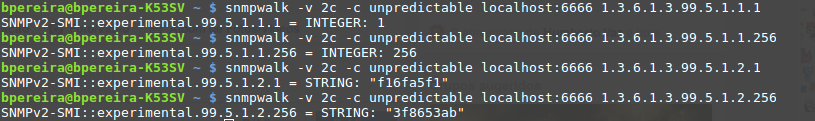
\includegraphics[width=\textwidth,height=\textheight,keepaspectratio]{resources/images/faseC/faseC.png}
 	\captionsetup{type=figure, width=0.8\linewidth}
	\caption{Testes}
\label{fig:faseB:teste} 
\end{center}




\clearpage
%---------------------------------------------------------------------------------------------------------------%
\section{Fase --- D}
%---------------------------------------------------------------------------------------------------------------%

Nesta fase, requere-se que se implemente a funcionalidade de refrescamento da
tabela de números hexadecimais, em intervalos de $\frac{1}{R}$ segundos, onde
\texttt{R} é o rácio de refrescamento em \emph{Hertz}.  Para o refrescamento,
considere-se $M_{T,K}$, onde $N=T$, $D=K$, e a matriz é circular, ou seja cada
coluna e cada linha é uma \emph{buffer} circular. Em consequência devem ser
aplicados os seguintes passos:

\begin{enumerate}
	\item $X$ é somatório do valor binário de todos os símbolos de chave de
		da operação de \emph{reset} (cada símbolo tem oito bits);

	\item$S_1$ é somatório do valor decimal de todos os dígitos $d_{i,j}$ de $M$ em
		que $i$ e $j$ são ambos pares;

	\item$S_2$ é somatório do valor decimal de todos os dígitos $d_{i,j}$ de $M$
		em que $i$ e $j$ são ambos ímpares;

	\item$C$ é igual ao resto da divisão inteira de $(S_1 + X)$ por
		$D$;\footnote{\emph{No enunciado $D$ estava trocado por $N$}}
                                                               
	\item$L$ é igual ao resto da divisão inteira de $(S_2 + X)$ por
		$N$;\footnote{\emph{ibidem}}

	\item Aplicar o refrescamento vertical   $v(C+1,1,M)$;

	\item Aplicar o refrescamento horizontal $h(L+1,1,M)$;

	\item Aplicar a operação de substituição $s(L+1,C+2,M)$;\footnote{\emph{No
		enunciado estava $s(L,C+2,M)$. No entanto, de acordo com a definição $L$ tem
	que ser maior ou igual a 1}}
\end{enumerate}


\newpage

As definições das operações $v$, $h$ e $s$ figuram a seguir:

\begin{itemize}
	\item$v(i, j, M_{T,K}$) 
	\item$h(i, j, M_{T,K}$)  
	\item $s(i, j, M_{T,K}$)
		\begin{itemize}
  \item Substituição da linha $i$ pelo resultado do \texttt{XOR} da linha: 
		\begin{itemize}
			\item $\begin{cases}
					\text{Se } i = 1~\text{Então}~i - 1 = T\\
					      i -1~\text{Caso contrário}
				     \end{cases}$ 
			\item $\begin{cases}
					\text{Se } i = T~\text{Então}~i + 1 = 1\\
					      i + 1~\text{Caso contrário}
				     \end{cases}$ 
		\end{itemize}
	\item  Substituição da coluna $j$ pelo resultado do \texttt{XOR} da coluna: 
		\begin{itemize}
			\item $\begin{cases}
					\text{Se } j = 1~\text{Então}~j - 1 = K\\
					      j - 1~\text{Caso contrário}
				     \end{cases}$ 
			\item $\begin{cases}
					\text{Se } j = K~\text{Então}~j + 1 = 1\\
					      j + 1~\text{Caso contrário}
				     \end{cases}$ 
		\end{itemize}
		\end{itemize}
\end{itemize}


As funcionalidades do \emph{refreshing} da tabela de números hexadecimais são
externas aos objetos da MIB, na medida que pertencem à classe
\emph{AgentHelper}, mas são partilhadas por processos que escrevem e leem dos
objetos, neste caso, a tabela de números hexadecimais. Assim, decidiu-se
adicionar 5 métodos e uma variável de instância na classe mencionada,i\.e,
os métodos \texttt{horizontal}, \texttt{vertical}, \texttt{substitution},
\texttt{refresh} e o tempo de refrescamento.

O tempo de refrescamento é calculado, logo na instanciação do
\emph{AgentHelper}, sendo mantido durante toda a execução do agente. O método
\texttt{refresh} aplica os cálculos já descritos acima, bem como a aplicação do
dos métodos \texttt{horizontal}, \texttt{vertical}, \texttt{substitution},
baseados em $v(i, j, M_{T,K}$), $h(i, j, M_{T,K}$), $s(i, j, M_{T,K}$),
respetivamente. Note-se que, se teve que se proceder à conversão de índices base
1, para índices base 0. Os valores da tabela da MIB são obtidos através de um
iterador e colocados num \emph{array} de \emph{strings} temporário, e das
manipulações numa matriz, obtida para o efeito da tabela, colocado de novo num
\emph{array} de \emph{strings} e com outro iterador alteram-se os valores com
os valores do último \emph{array}. 

\newpage

A \emph{Figura~\ref{fig:fasec:calcx}} representa o trecho de código onde foi
implementado o cálculo de $X$. Cada caractere em JAVA corresponde a um
\emph{byte}, ou seja, 8 bits, podendo somar-se diretamente ao estilo da
linguagem de programação C. 

\begin{center}
\begin{minted}{java}
for (int i = 0; i < this.getResetKey().length(); i++) {
	X += this.getResetKey().charAt(i);
}
\end{minted}
 	\captionsetup{type=figure, width=0.8\linewidth}
	\caption{Cálculo de $X$}
\label{fig:fasec:calcx} 
\end{center}


A \emph{Figura~\ref{fig:fasec:s1s2}} corresponde ao cálculo de $S_1$ e $S_2$,
vem como constrói uma matriz de inteiros, entre 0 e 15 (valores decimais
possíveis de um dígito hexadecimal), para as operações de deslocamento
e substituição.

\begin{center}
\begin{minted}{java}
for (int i = 0; i < N; i++) {
	for (int j = 0; j < D; j++) {

		m[i][j] = Integer.parseInt(seed[i].charAt(j) + "", 16);
		if (((i % 2) == 0) && ((j % 2) == 0)) {
			S1 += Integer.parseInt(seed[i].charAt(j) + "", 16);
		} else if (((i % 2) != 0) && ((j % 2) != 0)) {
			S2 += Integer.parseInt(seed[i].charAt(j) + "", 16);
		}

	}

}

\end{minted}
 	\captionsetup{type=figure, width=0.8\linewidth}
	\caption{Cálculo de $S_1$, $S_2$ e construção de matriz de inteiros}
\label{fig:fasec:s1s2} 
\end{center}

O cálculo de $C$ e $L$ figura abaixo.

\begin{center}
\begin{minted}{java}
int C = (S1 + X) % D;
int L = (S2 + X) % N;
\end{minted}
 	\captionsetup{type=figure, width=0.8\linewidth}
	\caption{Cálculo de $C$ e $L$}
\label{fig:fasec:} 
\end{center}


A \emph{Figura~\ref{fig:fasec:ops}} representa a aplicação das operações. 

\begin{center}
\begin{minted}{java}
vertical(C + 1, 1, N, m);
horizontal(L + 1, 1, D, m);
substitution(L + 1, C + 2, N, D, m);
\end{minted}
 	\captionsetup{type=figure, width=0.8\linewidth}
	\caption{Aplicação de \texttt{vertical}, \texttt{horizontal}
	e \texttt{substitution}}
\label{fig:fasec:ops} 
\end{center}

No método \texttt{main}, no ciclo infinito, aplica-se a operação de
\emph{refresh}, sendo o processo pausado durante o tempo de refrescamento
previamente calculado.

\clearpage
%---------------------------------------------------------------------------------------------------------------%
\section{Fase --- E}
%---------------------------------------------------------------------------------------------------------------%

Nesta última fase, implementou-se a funcionalidade de \emph{reset} da tabela de
número hexadecimais, à custa da receção de um \texttt{set-req} no agente,
enviado por um cliente SNMP, com um valor igual à chave de configuração. De
igual modo, pretende-se que a tabela de números hexadecimais seja atualizada com
os valores do ficheiro de sementes iniciais, sendo que após esta operação
o agente pause $R\times10$ segundos, antes de continuar com as operações de
refrescamento da tabela. 


Para implementar os requisitos, necessitou-se alterar a classe
\texttt{MOScalarFactory}, passando como argumento a instância de \texttt{Agent}
e \texttt{AgentHelper}, e por conseguinte, passar os mesmos argumentos
à instância da classe \texttt{ParamAuthReset}, que corresponde aos escalar da
chave da configuração.  Além disso, adicionou-se à classe \texttt{AgentHelper},
o método \texttt{reset}, um método para calcular o tempo de espera após
a operação de \emph{reset}, e também uma variável de condição associada a um
\emph{lock}, para servir de semáforo e uma \emph{flag} booleana para controlar
esse semáforo. 

Na classe \texttt{ParamAuthReset} também se fizerem algumas alterações. Para
o tratamento específico da receção do pedido de \emph{set-req} reescreveram-se
os métodos \texttt{prepare}, \texttt{commit}, \texttt{undo} e \texttt{cleanup}.
Estes métodos são invocados segundo o princípio 2PC (\emph{Two Phase Commit})
onde os valores recebidos de um \texttt{set-req} são validados no
\texttt{prepare} e alterados no \texttt{commit}. Se o \texttt{commit} falhar
todas as alterações são desfeitas no \texttt{undo} e o \texttt{cleanup} para
remover instâncias de objetos criados no processo.       

Com efeito, a comparação do valor de chave do pedido recebida foi implementada no método
\texttt{prepare}, obtendo-se a chave de configuração da instância de
\texttt{AgentHelper}, e aí são comparados os dois valores. Se os valores forem
diferentes, coloca-se o valor do estado do pedido como valor errado, sendo
depois tratado pelo método \texttt{commit}, \texttt{undo} e \texttt{cleanup},
nesta ordem. Note-se que se utilizaram as implementações dos métodos na
super-classe de \texttt{ParamAuthReset}, sendo adicionadas as funcionalidades
pretendidas após essa validação. Assim, quando o método \texttt{commit}
é invocado, se o valor do estado do pedido for igual ao código de valor errado,
o \texttt{commit} falha passando para o \texttt{undo}. Caso o valor do estado
for 0 (sucesso), é executado o que está no corpo do \texttt{commit}, ou seja um
\texttt{Runnable} (processo independente) que executa o método \texttt{reset} do
\texttt{AgentHelper}.  


Na classe \texttt{AgentHelper} modificou-se o método de refrescamento para
implementar o \emph{lock} da variável de condição, enquanto o valor da
\emph{flag} for verdadeira, sendo esta modificada pelo método \texttt{reset}. No
método \texttt{reset} da mesma classe, o algoritmo é o seguinte: quando o método
é invocado, a \emph{flag} é alterada para um valor verdadeiro, seguindo
o carregamento do ficheiro de sementes inicial, remoção do registo da tabela do
agente e criação e registo da nova tabela (conforme a sequência que está no
método \texttt{main} da fase C). Adicionalmente, coloca-se a \emph{flag}
a falso, e calcula-se e guarda-se novamente o tempo de espera, e por fim
sinalizámos o processo que tem o \emph{lock} da variável de condição para
proceder o seu normal funcionamento. 

No método \texttt{main}, no ciclo onde é feito o refrescamento, pausa-se
o processo durante o tempo de espera calculado, e após o o refrescamento da
tabela, alterámos o valor para 0. 

Considere-se também, que o \texttt{set-req} é assíncrono, e, durante uma
operação de refrescamento, o \emph{reset} pode ser despoletado. Neste caso ao
remover a tabela do registo, os valores que estão a ser obtidos no refrescamento
serão nulos. Para evitar uma exceção, colocou-se uma verificação na obtenção de
valores no método de refrescamento, onde caso um valor que seja obtido seja
nulo, o método termina imediatamente, deixando o método de \texttt{reset}
preencher a tabela.  




\subsection{Testes}

\begin{center}
 	
 	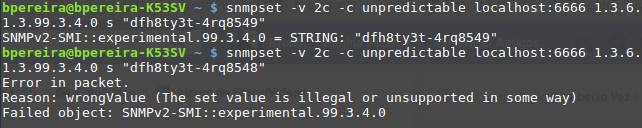
\includegraphics[width=\textwidth,height=\textheight,keepaspectratio]{resources/images/faseE/faseE.png}
 	\captionsetup{type=figure, width=0.8\linewidth}
	\caption{Testes}
\label{fig:faseB:teste} 
\end{center}




\clearpage

%---------------------------------------------------------------------------------------------------------------%
\section*{Conclusão\markboth{\MakeUppercase{Conclusão}}{}}
\addcontentsline{toc}{section}{Conclusão}


\subsection*{Trabalho futuro} 
\addcontentsline{toc}{subsection}{Trabalho Futuro}
% Implementar Better Effort ao invés de Best Effort


\clearpage
% ----------- %
%\bibauthoryear
\nocite{*}
\bibliography{IEEEabrv,referencias}
%\bibliography{referencias}{}
\bibliographystyle{IEEEtran}
%\bibliographystyle{ieeetr}
\clearpage
%%%%%%%%%%%%%%%%%%%%%%%%%%%%%%%%%%%%%%%%%%%%



\appendix 

%\part*{ANEXOS}
%\addcontentsline{toc}{section}{ANEXOS}
\part*{ANEXOS}
\addcontentsline{toc}{section}{ANEXOS}
%---------------------------------------------------------------------------------------------------------------%
\section{MIB}
\label{appendix:mib}
%---------------------------------------------------------------------------------------------------------------%
\begin{longlisting}
	\inputminted{text}{resources/images/faseA/mib.txt}
\label{listing:a}
\end{longlisting}









\end{document}

%%%%%%%%%%%%%%%%%%%%%%%%%%%%%%%%%%%%%%%%%%%%
%%%%%%%%%%%%%%%%%%%%%%%%%%%%%%%%%%%%%%%%%%%%
